\section{Diagramas de cajas y bigotes (boxplots)}

Un diagrama de caja (también, diagrama de caja y bigotes o box plot) es un
método estandarizado para representar gráficamente una serie de datos numéricos
a través de sus cuartiles. De esta manera, se muestran a simple vista la mediana
y los cuartiles de los datos, y también pueden representarse sus valores
atípicos, como se oberva en la Fig. (\ref{fig:boxplot}).

El diagrama de caja incluye los siguientes elementos:

\begin{itemize}
    \item rango (sin datos atípicos)
    \item datos atípicos
    \item rango intercuartil (también conocido como \textit{RIC})
    \item cuartiles ($Q_1$, $Q_2$ y $Q_3$)
    \item mediana ($Q_2$)
    \item mínimo y máximo
\end{itemize}

Para la elaboración de manera manual de este tipo de gráfico, primero se obtiene
la media de cada intervalo, y luego la mediana de la tabla de frecuencias en
general. Con estos datos, se utiliza la fórmula de la media de cada intervalo
elevado a la mediana.

\begin{enumerate}
\item Ordenar los datos y obtener el valor mínimo, el máximo, los cuartiles Q1,
Q2 y Q3 y el rango intercuartílico (\textit{RIC}):
\item Los \textit{bigotes}, las líneas que se extienden desde la caja, se
extienden hasta los valores máximo y mínimo de la serie o hasta 1,5 veces el
\textit{RIC}.
\item Cuando los datos se extienden más allá de esto, significa que hay valores
atípicos en la serie y entonces hay que calcular los límites superior e
inferior, \textit{Li} y \textit{Ls}.

Para ello, se consideran atípicos los valores inferiores a $Q_1-1.5 \cdot RIC$ o
superiores a $Q_3 + 1.5 \cdot RIC$.

\item Marcar como atípicos todos los datos que están fuera del intervalo ($Li$,
$Ls$).

\item Además, se pueden considerar valores extremadamente atípicos aquellos que
exceden $Q_1 - 3 \cdot RIC$ o $Q_3 + 3 \cdot RIC$.

\end{enumerate}

\subsection{Utilidad de los diagramas de cajas y bigotes}

\begin{itemize}
\item Proporcionan una visión general de la simetría de la distribución de los
datos; si la mediana no está en el centro del rectángulo, la distribución no es
simétrica.

\item Son útiles para ver la presencia de valores atípicos también llamados
outliers.

\item Pertenece a las herramientas de las estadística descriptiva. Permite ver
como es la dispersión de los puntos con la mediana, los percentiles 25 y 75 y
los valores máximos y mínimos.

\item Ponen en una sola dimensión los datos de un histograma, facilitando así el
análisis de la información al detectar que el 50\% de la población está en los
límites de la caja.
\end{itemize}

\begin{figure}[h!]
    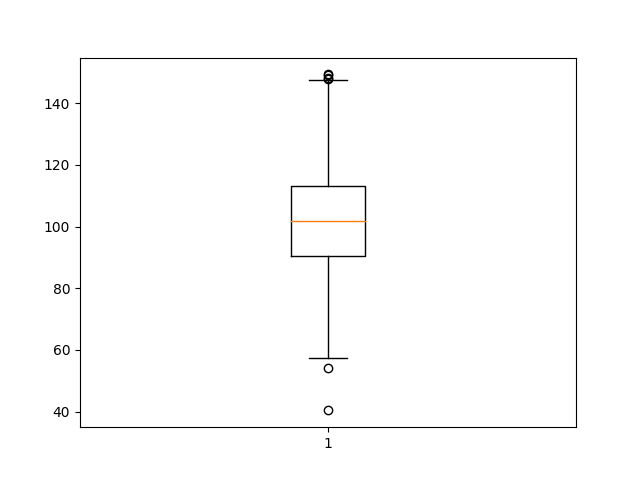
\includegraphics[scale=0.9]{figures/boxplot_test.png}
    \label{fig:boxplot}
    \caption{Diagrama de cajas para un experimento de números aleatorios con distribución normal}
\end{figure}
